\section{Theorie}
\label{sec:Theorie}


Im Folgenden wird der Operationsverstärker als zentrales Bauteil der verschiedenen Messreihen vorgestellt.
Darüberhinaus werden die damit verbundenen Schaltungen und deren verschiedene Funktionen dargestellt.
Im Übrigen wird der Unterschied zwischen idealem und realem Operationsverstärker näher beleuchtet.

\subsection{Der Operationsverstärker}

Ein Operationsverstärker ist ein spannungsgesteuerter Spannungsverstärker.
In Abbildung \ref{fig:OP}

\begin{figure}
    \centering 
    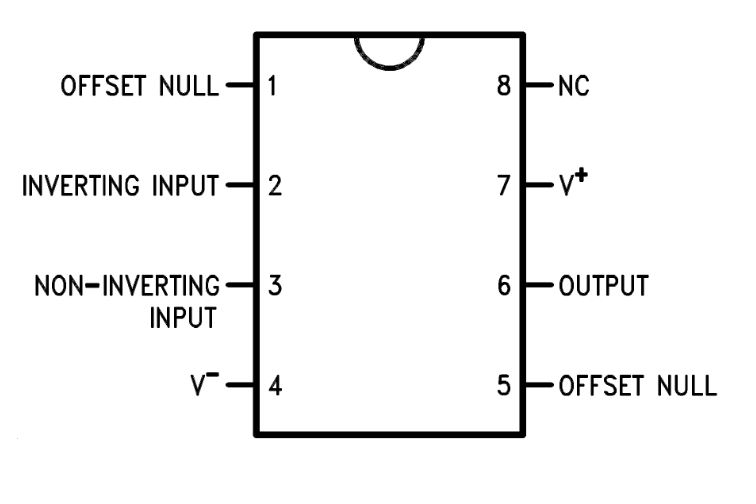
\includegraphics[width=.5\textwidth]{Bilder/OP.PNG}
    \caption{Anschlüsse eines LM741 Operationsverstärkers (\cite{LM741}).}
    \label{fig:OP}
\end{figure}

sind die Anschlüsse eines Operationsverstärkers vom Typ LM741 dargestellt.
Es gibt einen \textit{invertierenden} und einen \textit{nichtinvertierenden} Eingang.
Die Spannungsdifferenz an diesen Eingängen ergibt die Eingangsspannung.
Außerdem wird an die Anschlüsse $V^+$ und $V^-$ eine Versorgungsspannung gelegt.
Diese unterscheidet sich nur im Vorzeichen; ist also betragsmäßig gleich.
Am \textit{Output} befindet sich der Anschluss für die Ausgangsspannung.
Die Anschlüsse \textit{Offset Null} werden hier nicht benötigt, da die Offsets als vernachlässigbar klein angenommen werden.



Allgemein sorgt ein Operationsverstärker für eine Erhöhung der Eingangsspannung, wobei Ein- und Ausgangsspannung idealerweise in dem Zusammenhang
\begin{equation}
    U_A = v_0U_E 
\end{equation}
stehen.
$v_0$ gibt dabei den Verstärkungsfaktor der Leerlaufverstärkung an.
Dies gilt aber nur in dem nicht übersteuerten Bereich.
Der Bereich der Leerlaufverstärkung wird über die Höhe der Versorgungsspannung festgelegt.
Jenseits dieses Intervalls bleibt die Ausgangsspannung konstant bei der Versorgungsspannung.
In Abbildung \ref{fig:Kennlinie} ist eine typische Kennlinie dargestellt.

\begin{figure}
    \centering 
    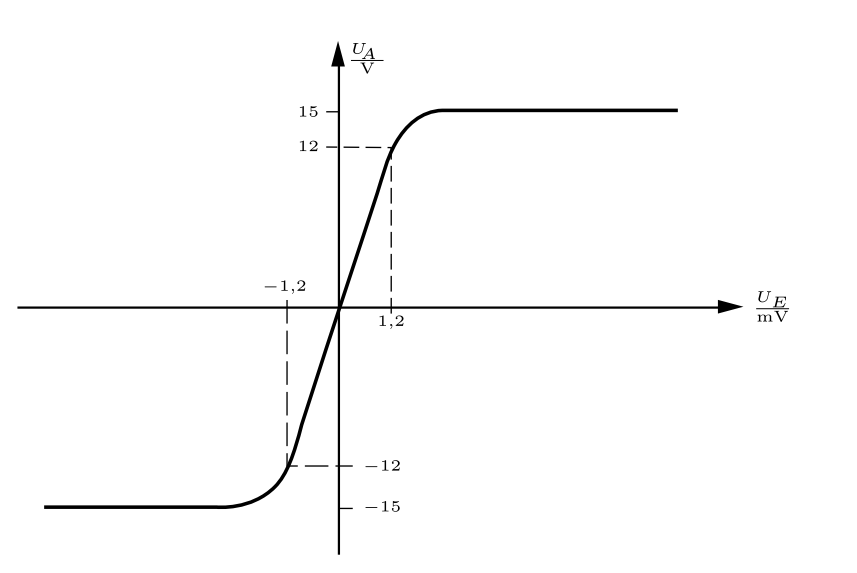
\includegraphics[width=.8\textwidth]{Bilder/Kennlinie.PNG}
    \caption{Beispiel für eine Kennlinie eines Operationsverstärkers (\cite[S.~99]{Clausert}).}
    \label{fig:Kennlinie}
\end{figure}

Ein idealer Operationsverstärker hat einen Eingangswiderstand von $R_E=\infty \si{\ohm}$ und einen Ausgangswiderstand von $R_A=\SI{0}{\ohm}$.
Die Verstärkung sollte auch unabhängig von weiteren Größen wie der Frequenz oder der Temperatur sein.
Im Realfall ist keine dieser Eigenschaften gänzlich erfüllt.
Der Eingangswiderstand hat die Größenordung $R_E > \SI{1}{\mega\ohm}$ und der Ausgangswiderstand befindet sich eher in dem Bereich $\SI{1}{\ohm} < R_A < \SI{1000}{\ohm}$.
Die Verstärkung beläuft sich auf Größenordungen von $v \propto 10^4$.



\subsection{Verschiedene Schaltungen}
Im Folgenden werden die im Versuch verwendeten Schaltungen aufgeführt.
Die Abbildungen der Schaltungen sind der Versuchsanleitung \cite{V51} entnommen.

\subsubsection{Invertierender Linearverstärker}
Die Schaltung eines invertierenden Linearverstärkers ist in Abbildung \ref{fig:Inv_Lin} dargestellt.
Über Rückkopplung an den invertierenden Eingang lässt sich der Verstärkungsfaktor
\begin{equation}
v_0 =-\frac{R_2}{R_1}    
\end{equation} 
über das Verhältnis der verbauten Widerstände bestimmen.
Dies ist aber nur im Idealfall erfüllt.
Der Verstärkungsfaktor der realen Schaltung ist frequenzabhängig und fällt ab einer bestimmten Grenzfrequenz $f_G$ ab.
Über 
\begin{equation}
    v = \frac{U_A}{U_E}
\end{equation}
lässt sich die tatsächliche Verstärkung berechnen.
Die Bandbreite kann dann über
\begin{equation}
    B = f_G \cdot v
\end{equation}
bestimmt werden.

\begin{figure}
    \centering 
    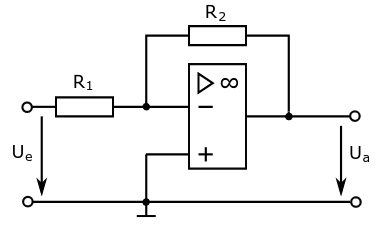
\includegraphics[width=.5\textwidth]{Bilder/Inv_Lin.png}
    \caption{Schaltbild eines invertierenden Linearverstärkers.}
    \label{fig:Inv_Lin}
\end{figure}

\subsubsection{Umkehr-Integrator und invertierender Differenzierer}

Über eine Gegenkopplung, in der Anstelle des Widerstandes ein Kondensator platziert wird, lassen sich Schaltungen realisieren, welche die Operation einer Integration und Differenziation durchführen.
Der Integrator ist in Abbildung \ref{fig:Um_Int} dargestellt.
Der Kondensator befindet sich also in dem Gegenkopplungszweig.
Unter Beachtung der Gleichungen
\begin{align*}
    U_E &= R \cdot I_E \\
    U_A &= U_C = \frac{1}{C}\int T_C \: \mathrm{d}t
\end{align*}
lässt sich die Eingangsspannung über
\begin{equation}
    U_A = -\frac{1}{RC} \int U_E \: \mathrm{d}t
\end{equation}
integrieren.




\begin{figure}
    \centering 
    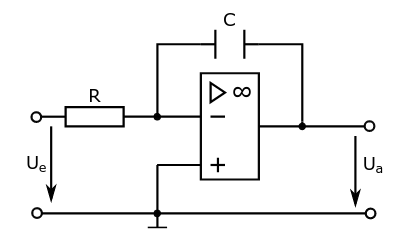
\includegraphics[width=.5\textwidth]{Bilder/Um_Int.png}
    \caption{Schaltbild eines Umker-Integrators.}
    \label{fig:Um_Int}
\end{figure}

Beim Differenzierer (Abbildung \ref{fig:Inv_Dif}) werden die Positionen von Widerstand und Kondensator getauscht.
Über die nun geltenen Gleichungen
\begin{align*}
    I_E &= \dot{Q} = C \cdot \dot{U_E} \\
    U_A &= R\cdot I_A
\end{align*}
lässt sich die Eingangsspannung über
\begin{equation}
    U_A = -RC \cdot \dot{U_E}
\end{equation}
differenzieren.

\begin{figure}
    \centering 
    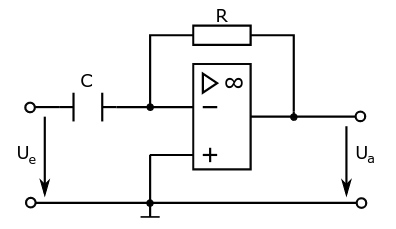
\includegraphics[width=.5\textwidth]{Bilder/Inv_Dif.png}
    \caption{Schaltbild eines invertierenden Differenzierers.}
    \label{fig:Inv_Dif}
\end{figure}


\subsubsection{Nichtinvertierender Schmitt-Trigger}

Das Schaltbild eines nichtinvertierenden Schmitt-Triggers ist in Abbildung \ref{fig:Schmitt} dargestellt.

Zu beachten ist, dass im Gegensatz zu den vorherigen Schaltungen, der Gegenkopplungszweig im nicht invertierenden Eingang mündet.
Über diesen feinen aber wichtigen Unterschied erhält die Schaltung die Funktionen eines Schalters, welcher ab einer gewissen Schwellenspannung die Ausgangsspannung schlagartig ändert.
Dieses Verhalten ist in Abbildung \ref{fig:Kenn_Schmitt} als Kennlinie verdeutlicht.
Der theoretisch zu erwartene Wert für die Schwellenspannung lässt sich über
\begin{equation}
    U_{E \: \text{ab}} = \frac{R_1}{R_2} U_{A\text{max}}
    \label{eq:schmitt}
\end{equation}
bestimmen.
$U_{A \: \text{max}}$ beschreibt den Maximalwert der Ausgangsspannung.

\begin{figure}
    \centering 
    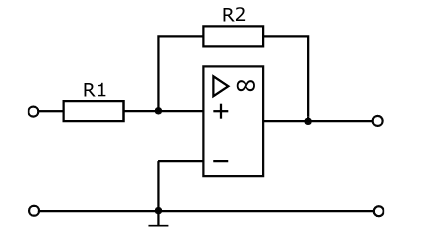
\includegraphics[width=.5\textwidth]{Bilder/Schmitt.png}
    \caption{Schaltbild eines nichtinvertierenden Schmitt-Triggers.}
    \label{fig:Schmitt}
\end{figure}

\begin{figure}
    \centering 
    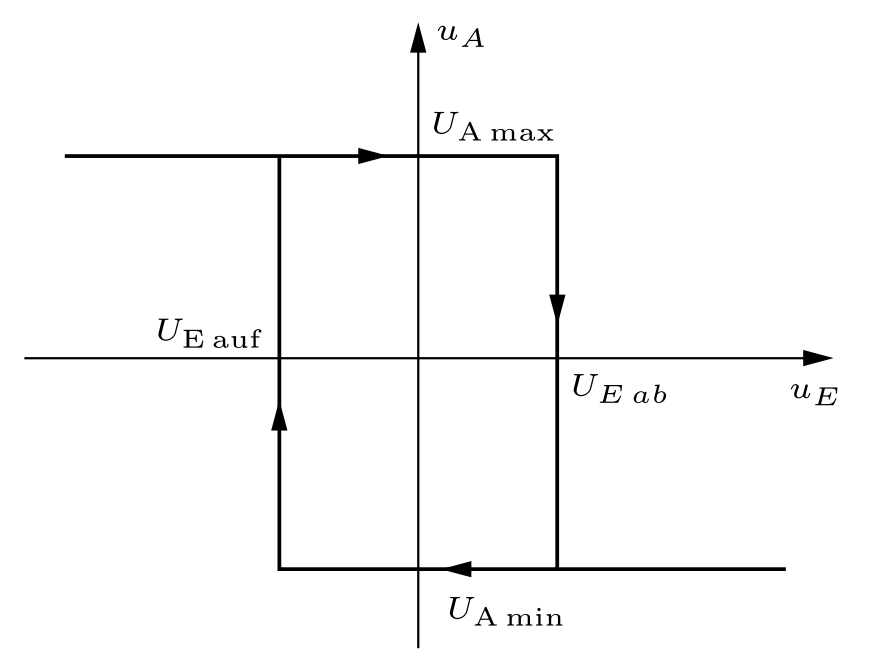
\includegraphics[width=.5\textwidth]{Bilder/Kenn_Schmitt.PNG}
    \caption{Kennlinie eines nichtinvertierenden Schmitt-Triggers (\cite[S.~115]{Clausert}).}
    \label{fig:Kenn_Schmitt}
\end{figure}

\subsubsection{Signalgenerator}
Es lassen sich der invertierende Integrator und der Schmitt-Trigger zu einem Signalgenerator kombinieren.
Eine solche Schaltung ist in Abbildung \ref{fig:Signal} einzusehen.
Der Schmitt-Trigger tranformiert jedes periodisches Signal in eine Rechteckspannung.
Diese wird über den Integrator zu einer Dreiecksspannung integriert, welche wieder mit dem Schmitt-Trigger rückgekoppelt wird.
Über die Rückkopplung des Integrator-Ausganges zu dem Schmitt-Trigger-Eingang fängt das system autonom an zu schwingen.
Es sind also keine externen Eingangssignale notwendig.
So hat das Ausgangssignal dieser selbstinduzierenden Schwingung die Form einer Dreiecksspannung.
Die theoretische Frequenz und Amplitude dieses Signals lassen sich über
\begin{equation}
    f = \frac{R_2}{4CR_1R_2}
    \label{eq:sig_f}
\end{equation}
und 
\begin{equation}
    A = \frac{R_1}{R_2}\cdot U_{A \: \text{max}}
    \label{eq:sig_a}
\end{equation}
berechnen.

\begin{figure}
    \centering 
    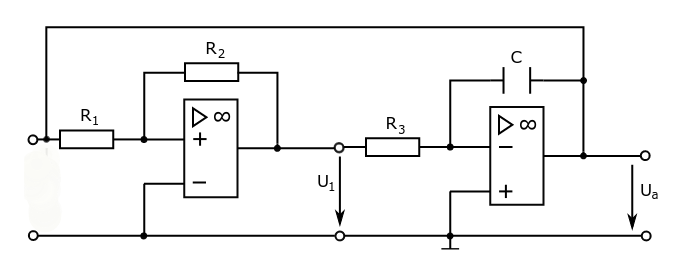
\includegraphics[width=.9\textwidth]{Bilder/Signal.png}
    \caption{Schaltbild eines Signalgenerators aus der Reihe eines nichtinvertierenden Schmitt-Triggers und eines Umker-Integrators.}
    \label{fig:Signal}
\end{figure}
%In knapper Form sind die physikalischen Grundlagen des Versuches, des Messverfahrens, sowie sämtliche für die Auswertung erforderlichen Gleichungen darzustellen. (Keine Herleitung)

%(eventuell die Aufgaben)

%Der Versuchsaufbau: Beschreibung des Versuchs und der Funktionsweise (mit Skizze/Bild/Foto)
